\scanpage{9}
De même, pour la \deleted{\unsure{définition}} vérification de l'associativité,
on n'a utilisé la formule de projection et la
formule d'échange que dans le cas
\diagram{\begin{tikzcd}[column sep=small,row sep=large]
&X\times Y\times P\arrow[dl]\arrow[dr]&\\
X\times P\arrow[dr,no head]&&Y\times P\arrow[dl,no head]\\
&P&
\end{tikzcd}}
mais pour vérifier que les $\unsure{\delta_X|\Delta_X}^{\unsure{s|?}}$ sont des
unités, on en avait besoin aussi dans un cas
\diagram{\begin{tikzcd}[column sep=small,row sep=large]
&X\times Y\arrow[dl]\arrow[dr,hook]&\\
X\arrow[dr,hook,"\mathrm{diag.}"']&&X\times X\times Y\arrow[dl,"\mathrm{proj}"]\\
&X\times X&
\end{tikzcd}}

\figure{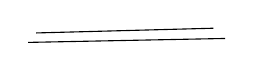
\begin{tikzpicture}\draw (0,0)--(2.5,.05);\draw (.1,.12)--(2.35,.18);\end{tikzpicture}}

Définissons le foncteur $\varphi$, en définissant pour
tt $X,Y\in\operatorname{Ob}\mathcal V$ une application
\[
\varphi_{X,Y}:\operatorname{Hom}_{\mathcal V}(X,Y)\longrightarrow
\operatorname{Hom}_{\mathcal V^A}(X,Y)=A(X\times Y)
\]
Soit donc $f:X\longrightarrow Y$ dans $\mathcal V$, on en définit
un hom graphe
\[
\Gamma_f=(\operatorname{id}_X,f):X-X\times Y
\]
d'où
\[
A(\Gamma_f)_*:A(X)\longrightarrow A(X\times Y)
\]
Posons alors
\[
\deleted{\unsure{A}}\quad\varphi_{X,Y}(f)=A(\Gamma_f)_*(1)
\]
\mspage{8}
